 \documentclass[ngerman]{scrartcl} %lädt die Dokumentklasse
                                %Artikel von Koma-Skript, als Option
                                %übergebe ich, dass ich die Trennung
                                %nach neuer deutscher Rechtschreibung
                                %wünsche
\usepackage[utf8]{inputenc}
\usepackage[ngerman]{babel}
\usepackage{color}
\usepackage[T1]{fontenc}
\usepackage[pdfborder={0 0 0}]{hyperref}
\usepackage[a4paper,lmargin={4cm},rmargin={2cm},
tmargin={2.5cm},bmargin = {2.5cm}]{geometry}
\usepackage{amssymb}
\usepackage{graphicx}
\usepackage{amsthm}
\usepackage{graphicx}
\usepackage{url} 
\usepackage{listings}
\usepackage{acronym} 

\begin{document}
\tableofcontents
\newpage
 
\section{Einleitung}        
\label{sec:Einleitung-1}   

In den letzten Jahren konnten aufgrund technologischer Entwicklungen immer mehr Geräte entwickelt werden, die in den verschiedensten Bereichen des täglichen Lebens eingesetzt werden. Diese Entwicklungen betreffen dabei meist die Leistungsfähigkeit, Konnektivität oder Größe der Geräte, sodass sie in immer mehr und unterschiedlicheren Bereichen eingesetzt werden können. Ein Begriff der in den letzten Jahren für dieses Phänomen immer häufiger genutzt wurde, ist das ``\ac{IoT}'' zu deutsch ``Das Internet der Dinge''. Mit dem \ac{IoT} wird beschrieben, dass immer mehr Geräte mit dem Internet verbunden sind und Daten austauschen. Im Rahmen dieser Entwicklung sind verschiedenste Nutzungsszenarien umgesetzt worden, die das tägliche Leben erleichtern oder automatisieren sollen. Diese Studienarbeit wird sich im folgenden mit einem speziellen Szenario befassen, welches unter anderem durch den Onlinehändler Amazon umgesetzt wurde.

Das Szenario umfasst sogenannte ``Amazon Dash Buttons''. Diese Buttons sind kleine Geräte, welche an unterschiedlichen Stellen in der Wohnung des Kundens angebracht werden können und über einen Druckknopf verfügen. Nach einer Konfiguration durch den Benutzer kann mithilfe eines Drucks auf den Sensor ein zuvor ausgewähltes Produkt bestellt werden. Ein Beispiel wäre das nachbestellen von Waschpulver. So könnte der Button an der Waschmaschine befestigt sein und bei einem geringen Vorrat an Waschpulver wird der Button betätigt und das ausgewählte Waschpulver innerhalb der nächsten Tage geliefert. So entfällt für den Nutzer der händische Bestellvorgang, da dieser automatisch durch den Button und Amazon durchgeführt wird. Dieses Beispiel lässt sich natürlich auf verschiedene andere Möglichkeiten übertragen, so könnten auch Dinge, wie Kaffee, Zahnpasta, Tierfutter, Getränke oder ähnliches nachbestellt werden. Dem Nutzer wird eine Vereinfachung des Kaufprozesses versprochen und der Händler bindet den Kunden stärker an sich, da der Button direkt bei Amazon bestellt. 
Die Studienarbeit setzt sich zum Ziel eine Untersuchung des Amazonproduktes durchzuführen und die Machbarkeit und Umsetzung einer offeneren Lösung zu prüfen. 

    

\newpage

\section{Aufgabenstellung}
\label{sec:Aufgabenstellung-1}

Wie bereits in der \nameref{sec:Einleitung-1} erwähnt, soll sich diese Studienarbeit mit der Untersuchung des Amazon Dash Buttons beschäftigen und eine Alternative entwickeln. Da bereits während der Recherche vor Projektbeginn herausgefunden werden konnte, dass der Button in der Standardkonfiguration nur mit den Services von Amazon zusammenarbeiten kann, soll eine offenere Lösung entwickelt werden. Mit einer offeneren Lösung wird im Rahmen dieser Studienarbeit eine Möglichkeit definiert, die dem Kunden einen ähnlichen Funktionsumfang anbietet. Ein grundlegender Unterschied ist jedoch im Bestellprozess vorhanden. Während die Lösung von Amazon eine direkte Bestellung bei Amazon auslöst, soll die offenere Lösung eine Einkaufsliste mit Produkten erstellen. 

Der Nutzer soll dann über ein Webfrontend die Möglichkeit haben den Einkaufszettel zu betrachten und dann die entsprechenden Produkte bei seinem bevorzugten Händler zu bestellen. So kann es auch möglich sein, dass auch Produkte geführt werden, die der Nutzer nicht online bestellen kann. Der Vorteil bei dieser Lösung liegt darin, dass der Nutzer nicht an einen Händler und dessen Preise gebunden ist, sondern die Preise vergleichen und einen entsprechenden Händler, der seinen persönlichen Kriterien entspricht, wählen kann. 
Im Rahmen dieses Ziels müssen verschiedene Komponenten entwickelt werden, die im Rahmen der Lösung zusammenarbeiten. Diese Komponenten lassen sich unter folgenden Kategorien zusammenfassen:
\begin{itemize}
\item Entwicklung von Buttons 
\item Entwicklung eines Frontends zur Nutzerinteraktion
\item Entwicklung eines Backends zur Verarbeitung von Frontendeingaben und der Eingabe von Buttons 
\end{itemize}
Die Entwicklung von Buttons lässt sich dabei in zwei Teile aufteilen. Zum einem soll der Amazon Dash Button betrachtet und analysiert werden. In diesem Rahmen soll sowohl die Einrichtung und Konfiguration als auch die Kommunikation untersucht werden. In Folge dessen soll weiterhin geprüft werden, ob der Button auch für die offene Lösung genutzt werden kann und dabei kein Produkt bei Amazon bestellt. Weiterhin sollen mithilfe von Mikrokontrollern eigene Buttons entwickelt werden, die ebenfalls ein Signal an den entsprechenden Empfänger absenden können. Bei den Buttons steht die Funktionalität und die Prüfung der Machbarkeit des Projektes im Vordergrund. Die Gestaltung der Buttons spielt keine priorisierte Rolle. 


Weiterhin muss ein Frontend entwickelt werden, welches die Nutzerinteraktion ermöglicht. Das Frontend soll zur Übersicht der Einkaufsliste genutzt werden, aber auch die Verwaltung der Buttons und andere anfallende Verwaltungsfunktionen sollen ermöglicht werden. 
Um eine Kommunikation zwischen Frontend und den Buttons zu gewährleisten, muss ein Backend entwickelt werden, welches über Schnittstellen die Kommunikation gewährleistet und die Eingaben entsprechend verarbeitet. 
Als Ergebnis des Projektes soll möglichst ein eigener Button entstanden sein, der mithilfe des Backends und Frontends dem Nutzer ermöglicht einen ähnlichen, aber offeneren Prozess, wie bei Amazon, zu nutzen. Weiterhin soll zumindest der Amazon Dash Button untersucht worden sein und wenn möglich miteingebunden sein. Abschließend soll ein Fazit gezogen werden, inwiefern das Projekt umsetzbar ist. 

\newpage

\section{Theorie}        
\label{sec:Theorie-1}  

Im Rahmen dieser Arbeit wurden verschiedene Technologien und Prinzipien eingesetzt. Auf diese soll in den folgenden Unterkapiteln eingegangen werden, damit eine theoretische Grundlage vorhanden ist. 

\subsection{\ac{UDP}}
\label{sec:UDP-1}

\ac{UDP} steht für ``User-Datagram-Protocol'' und ist ein verbindungsloses Transportprotokoll. Im \ac{OSI}-7-Schichten Modell arbeitet es auf der Transportebene und ist für die Zustellung von Netzwerkpaketen von einem Sender zu einem Empfänger zuständig. Im Vergleich zum Transportprotokoll \ac{TCP}, welches verbindungsorientiert arbeitet, ist es wesentlich einfacher zu verarbeiten, da beispielsweise der Header bei den einzelnen Datenpaketen wesentlich kleiner ist. Allgemein ist es sehr minimal gehalten und dadurch sehr einfach zu implementieren und für sehr einfache Anwendungszwecke geeignet. Allerdings ist auch zu erwähnen, dass es keine Empfangsbestätigung gibt und die Daten nach dem Absenden nicht weiter kontrolliert werden. Somit können die Daten auch im Netzwerk verloren gehen und es wird nicht bemerkt. \\
Der einfache Header des \ac{UDP} Protokolls besteht nur aus vier Attributen. Diese jeweils 16 Bit großen Felder enthalten den Quellport, den Zielport, die Checksumme zur Überprüfung des Inhalts und die Länge des gesamten Pakets. Insgesamt ist der Header somit 8 Byte groß. (vgl. \cite{ElektronikKompendium.}\cite{.}\cite{.23.02.2016})
 

\subsection{\ac{TCP}}
\label{sec:TCP-1}

\ac{TCP} ist ein verbindungsorientiertes Protokoll, dass im \ac{OSI}-7-Schichten Modell auf der vierten Ebene (Transport) einzuordnen ist. Im sogenannten \ac{TCP}/\ac{IP} Protokollstapel ist es in der dritten von vier Schichten zu finden. Bei einer Übertragung von Daten über \ac{TCP} übergibt die genutzte Anwendung den Datenstrom an das Protokoll und empfängt ihn auch wieder von dort. Für die Übertragung ist dementsprechend \ac{TCP} zuständig. 
Die Hauptaufgaben des Protokolls sind daher die Aufteilung und die Zusammensetzung der Daten von entsprechend vielen Paketen (Segmentierung), das Management der Verbindung und ein entsprechendes Fehlerhandling, welches das korrekte Empfangen von Paketen überwacht. Das Fehlerhandling nutzt eine positive Bestätigung aller Pakete. Dies bedeutet, dass nur nicht vorhandene Pakete erneut angefragt werden, ansonsten davon ausgegangen wird, dass die Daten beim Empfänger angekommen sind. Diese Technologie sorgt dafür, dass die Daten auf jeden Fall ankommen, sofern die Verbindung nicht gestört wird (vgl. \cite{.c}\cite{.22.11.2016}).

Der Header eines \ac{TCP} Pakets besteht aus 20 Bytes, jedoch kann dieser auch noch erweitert werden, sodass noch einige zusätzliche Bytes in den Header geschrieben werden. Zu den zwingend notwendigen Daten gehört unter anderem der Port auf dem das Paket empfangen wird und der Port über den das Paket gesendet wird. Zudem wird die Nummer im aktuellen Paketstrom benötigt. Zudem wird eine Prüfsumme und Quittierungsnummer mitgegeben, welche zur Kontrolle und Bestätigung genutzt werden (vgl \cite{.c}).


\subsection{Webserver: Nginx}
\label{sec:Webserver: Nginx-1} 
 
\subsection{Arduino}
\label{sec:Arduino-1} 

Die Bezeichnung Arduino steht für eine Technologie, die sowohl aus einer Hardwarekomponente als auch aus einer Softwarekomponente besteht. Zudem gibt es zwei Unternehmen, die in ihrem Namen den Begriff Arduino tragen und in Zusammenhang mit der Technologie stehen. Zum einem gibt es die Arduino LLC, die die Gruppe der Gründer der Plattform bezeichnet. Des Weiteren gibt es die Arduino S.r.l., das die Firma bezeichnet, die anfangs allein die Arduinoboards produzierte und dann auch verkaufte. Die Arduinoplattform wurde ursprünglich entwickelt, um Anfängern den Einstieg in die Mikrokontrollerprogrammierung zu vereinfachen. 

Grundsätzlich besteht die sogenannte Arduinoplattform aber sowohl aus der Hardware als auch der Software. Die Hardware umfasst mittlerweile verschiedene Mikrokontroller beziehungsweise Einplatinencomputer, welche für verschiedene Anwendungszwecke genutzt werden können. Die entsprechende Nutzung wird mithilfe der richtigen Programmierung erreicht. Dafür kann der Softwareteil der Lösung genutzt werden, welches aus einer \ac{IDE}  besteht und das Schreiben von Programmen vereinfacht. Zudem wird über diese \ac{IDE} auch die Kommunikation mit dem Mikrokontroller realisiert. Diese Entwicklungsumgebung eignet sich für diverse Mikrokontroller, sofern entsprechende Treiber verfügbar sind, können auch Boards genutzt werden, die nicht direkt mit Arduino zusammenhängen. Zudem kann in verschiedenen Programmiersprachen entwickelt werden, beispielsweise C oder C++. (vgl. \cite{.h,.f,.e,.i,.g,online.})
Die komplette Plattform ist open source, auch wenn die Hardware natürlich erworben werden muss. 



\subsection{Python}
\label{src:Python-1}

\subsection{WLAN-Chipsatz}
\label{sec:WLAN-CHipsatz-1} 

\subsection{Frontendtechnologien}
\label{sec:Frontendtechnologien-1}
 
\subsection{\ac{REST}}        
\label{sec:REST-1}  

\cite{Tilkov.2015}
  
\newpage
 
\section{Beschreibung der Hardware}        
\label{sec:Beschreibung der Hardware-1}  

In den folgenden Kapiteln wird die ausgewählte Hardware des Projektes vorgestellt. Dabei wird zuerst auf die technischen Merkmale eingegangen und dann auf den genauen Verwendungszweck im Projekt. 

\subsection{Raspberry PI}        
\label{sec:Raspberry PI-1} 


\subsubsection{Vorstellung des Raspberry PI}        
\label{sec:Vorstellung des Raspberry PI-1} 

Das Raspberry PI ist ein Einplatinencomputer, den es in verschiedenen Ausführungen gibt. Je nach Ausführung variieren die Ausstattungsmerkmale. Zu den Grundsätzlichen Ausstattungsmerkmalen gehören eine CPU, unterschiedlich viel RAM und eine iGPU Einheit. Er wurde von der Raspberry PI Foundation entwickelt und hatte das ursprüngliche Ziel einen günstigen Computer für den Schulunterricht bereitzustellen. Daher ist es auch möglich eine vollständige Linux Distribution als Betriebssystem zu nutzen und es wurde sogar eine speziell angepasste Distribution veröffentlicht, die Raspbian bezeichnet wird. 
Aufgrund der verschiedenen Möglichkeiten wird er aber mittlerweile auch in vielen anderen Anwendungsgebieten genutzt. Insbesondere die neueren Modelle, die mit mehreren USB Ports, \ac{GPIO} Pins, einem Ethernet Port und weiteren Anschlüssen ausgestattet sind, werden auch in verschiedensten Projekten privater Personen genutzt. Ein weiteres Merkmal ist die Größe des Raspberry PI's, die mit maximal 93mmx63.5mmx20mm sehr klein ausfällt. Zusätzlich gibt es diverses, bereits für den Raspberry PI ausgelegtes, Zubehör, welches weitere Erweiterungsmöglichkeiten bietet. So gibt es Kameras, Gehäuse, kleine Displays und WLAN Sticks, die den Funktionsumfang erweitern. So wurden bereits diverse Projekte vorgestellt, die zeigen, dass die Einsatzmöglichkeiten des Raspberry Pis wesentlich größer sind. (vgl. \cite{.28.12.2016} \cite{.28.01.2017})
\\
\begin{figure}[!htb]
	\centering
	\includegraphics[scale=0.5]{Raspberry-Pi-2-web.png}
	\caption[RaspberryPi Modell 2 B]{RaspberryPi Modell 2 B+,\\ Quelle: https://www.raspberrypi.org/wp-content/uploads/2016/02/Raspberry-Pi-2-web.jpg}
\end{figure}


\subsubsection{Verwendung im Projekt}        
\label{sec:Verwendung des Raspberry PI-1} 
Der Raspberry PI wird für das Projekt genutzt, um einen zentralen Server bereitzustellen. Aufgrund der technischen Merkmale kann zeitgleich ein Webserver und ein Datenbankserver betrieben werden. Zudem kann über die USB Anschlüsse ein WLAN Stick angeschlossen werden, sodass die Buttons über das WLAN Netzwerk des Raspberry PIs zum zentralen Server kommunizieren können. Dazu muss mithilfe eines Skriptes der WLAN Stick von einem Empfänger zu einem Sender bzw. Access Point umfunktioniert werden. Um die dann eingehenden Nachrichten der Buttons empfangen zu können, muss zudem noch ein entsprechendes Skript im Hintergrund laufen, dass die Daten empfängt. Aufgrund von mehreren parallel laufenden Prozessen (Webserver, Datenbankserver, WLAN Skript und Skripte zum Empfangen der Daten) wird einiges an Rechenleistung benötigt, die der Raspberry Pi allerdings aufbringen kann. 

Der Webserver auf dem Raspberry Pi wird dabei sowohl für das Frontend als auch für das Backend benötigt werden. Das Frontend soll dem Nutzer die Möglichkeit geben, die Liste von Waren zu verwalten und die Buttons zu konfigurieren bzw. Hilfestellung zur Einrichtung zu geben. Das Backend des Servers wird unter anderem aus einer \ac{REST} \ac{API} bestehen, die sowohl die Anfragen des Webservers verarbeitet als auch die Anfragen an die Datenbank im allgemeinen. 
Der Datenbankserver im Hintergrund wird die benötigte Datenbank entsprechend verwalten. 
\newpage

\subsection{``Pretzelboard''}        
\label{sec:Pretzelboard-1} 

\subsubsection{Vorstellung des ``Pretzelboard''}        
\label{sec:Vorstellung des ``Pretzelboard''} 
Das ``Pretzelboard'' ist ein sogenanntes Elektronikmodul, dass unter verschiedenen Namen bekannt ist. Neben ``Pretzelboard'' ist der Name ``NanoESP-Board'' ebenfalls bekannt. Die Besonderheit des Boards ist ein bereits angeschlossenes WLAN Modul, welches sowohl als Sender als auch Empfänger arbeiten kann. Da es zudem den gleichen Mikrocontroller wie das bekanntere Mikrocontrollerboard ``Arduino Uno'' nutzt, kann die Entwicklungsumgebung von Arduino zur Entwicklung von Software genutzt werden. 
Der Vorteil der bereits erfolgten Kombination und Verdrahtung von WLAN Modul und Mikrocontroller liegt darin, dass der Nutzer dies nicht mehr machen muss und somit wesentlich weniger Kenntnisse vorausgesetzt werden müssen. (vgl. \cite{.b}\cite{.kafka}\cite{FranzisVerlagGmbH.27.11.2015})


\subsubsection{Verwendung im Projekt}        
\label{sec:Verwendung des ``Pretzelboard''} 
Das ``Pretzelboard'' wird im Projekt als Button genutzt. Sowohl die kleine Größe als auch die bereits vorhandene WLAN Funktionalität sorgen dafür, dass sich das Board dafür besonders gut eignet. Aufgrund der Tatsache, dass es sich bezüglich der Programmierung nicht von einem Arduino Board unterscheidet, besteht die Möglichkeit, dass auf das Wissen und den Support einer bereits größeren Community zurückgegriffen werden kann. 
Da sich das Board zudem auf ein Elektroniksteckboard setzen lassen kann, ist auch die Verbindung mit einem Button und Statusleuchten möglich. Nach der erfolgreichen Montage kann dann das entsprechende Programm aufgespielt werden und bei vorhandener Stromversorgung kann die entsprechende Nachricht über das WLAN Netzwerk an den Empfänger gesendet werden. Das Pretzelboard kommuniziert diese Nachricht mithilfe des zuvor bereits erwähnten Protokolls \nameref{sec:UDP-1}.

\begin{figure}[!htb]
	\centering
	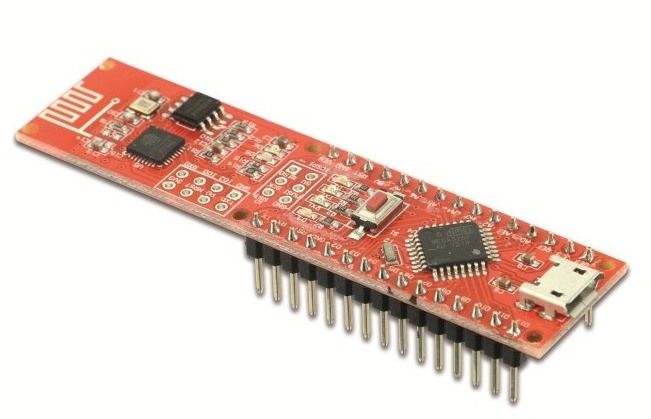
\includegraphics[scale=0.4]{pretzel.jpg}
	\caption[``Pretzelboard'']{``Pretzelboard'',\\ Quelle: http://cdn.pollin.de/article/xtrabig/X880281.2.JPG}
\end{figure}

\newpage

%Bild vom fertigen Button
\newpage

\subsection{ESP8266 Lua}
\label{sec:ESP8266}

\subsubsection{Vorstellung des ESP8266 Lua}        
\label{sec:Vorstellung des ESP8266} 

Der ESP8266 Lua ist ein Entwicklungsboard, welches bereits ein integriertes WLAN Modul besitzt und mit einem TCP/IP Stack ausgestattet ist. Einer der vorgesehenen Einsatzzwecke ist unter anderem das Internet of Things. Das Board kann zudem mit Steckbrett arbeiten und bietet daher ähnliche Möglichkeiten, wie das bereits erwähnte \nameref{sec:Pretzelboard-1}. Zudem ist es möglich, dass die Software für das ESP8266 Lua Entwicklungsboard ebenfalls über die Arduino IDE entwickelt werden kann. Allerdings sind technische Unterschiede zum Pretzelboard vorhanden, was dazu führt, dass andere Treiber genutzt werden müssen. 
Diese können nachinstalliert werden und stehen dann zur Nutzung des Boards bereit. (vgl. \cite{Carius.15.01.2017}\cite{.d})

\subsubsection{Verwendung im Projekt}        
\label{sec:Verwendung des ESP8266} 
Das Board wird im Rahmen des Projektes als weiterer Button genutzt. Es bietet sich für diese Funktion an, da es ebenfalls recht klein ist und alle benötigten Funktionen bereits vorhanden sind. Neben den vorhandenen Funktionen ist auch die Möglichkeit vorhanden, dass eine bereits durch das Bretzelboard bekannte Entwicklungsumgebung genutzt werden kann. Das bietet die Möglichkeit, dass statt des UDP Protokolls das bereits erwähnte \nameref{sec:TCP-1} Protokoll ausprobiert werden kann. 
Der Aufbau des Boards soll ebenfalls durch ein Elektroniksteckboard umgesetzt werden. Dazu wird das Board auf eben dieses Steckboard gesetzt und mit einem Button, Statusleuchten und entsprechenden Kabeln verbunden. Nach der Betätigung des Buttons wird das Board geweckt und eine Funktion schickt ein entsprechendes Datenpaket an einen Empfänger.
\newpage

%Bild vom fertigen Button 

\subsection{Amazon Dash Button}
\label{sec:Amazon Dash Button}

\subsubsection{Vorstellung des Amazon Dash Buttons}        
\label{sec:Vorstellung des Amazon Dash Buttons} 

\subsubsection{Untersuchung des Amazon Dash Buttons}        
\label{sec:Untersuchung des Amazon Dash Buttons} 

\subsubsection{Verwendung des Amazon Dash Buttons im Projekt}        
\label{sec:Verwendung des Amazon Dash Buttons im Projekt} 

%Bild vom Button 
\newpage

\section{Umsetzung des Projektes}        
\label{sec:Umsetzung des Projektes-1}  

\subsection{Architektur und Zusammenarbeit der Komponenten}        
\label{sec:Architektur und Zusammenarbeit der Komponenten-1} 

Mithilfe der Technologien und Softwarelösungen, die in Kapitel \ref{sec:Theorie-1} erläutert worden sind, und der Hardware, die in Kapitel \ref{sec:Beschreibung der Hardware-1} vorgestellt wurde, konnten die verschiedenen Komponenten, die bereits in der Aufgabenstellung (vgl. Kapitel \ref{sec:Aufgabenstellung-1}) genannt worden sind, umgesetzt werden. 
Im folgenden soll ein Überblick über die Zusammenarbeit der einzelnen Komponenten gegeben werden, bevor in den folgenden Kapiteln auf die genaue Entwicklung der einzelnen Komponenten eingegangen wird. 

Für den Nutzer gibt es ein Webfrontend, welches mithilfe eines Nginx Webservers (vgl. Kapitel {sec:WebserverNginx-1}) realisiert wird. Dieses Webfrontend greift auf ein \ac{REST} \ac{API}-Backend zurück, welches in \ac{PHP} geschrieben wurde und ebenfalls über den Nginx realisiert wird. Mithilfe dieses Backends werden die verschiedenen \ac{API} Routen realisiert, die dann den Zugriff auf die Datenbank organisieren. Das Backend besteht ebenfalls aus einigen Skripten, die in Python\ref{src:Python-1}) geschrieben sind. Diese Skripte organisieren die Kommunikationsendpunkte für die Buttons, indem sie auf die entsprechende Kommunikationsports für die Datenpakete lauschen und die Daten dann verarbeiten. 

Neben der Kommunikation wird ebenfalls ein Teil der \ac{REST} \ac{API} in Python realisiert. Dieser Teil ermöglicht sowohl den Status der Skripte, die die Kommunikation organisieren, abzufragen als auch die Skripte neu zu starten, sollte ein Skript nicht gestartet sein oder ein Fehler aufgetreten sein. Diese Daten werden ebenfalls für das Webfrontend verwendet. 
Die Buttons, als weitere Komponente, werden durch verschiedene Hardwareelemente realisiert. Mithilfe entsprechender Programme, die auf die Controller geladen werden, stellen sie eine Verbindung zu den definierten Kommunikationspunkten her. Über dieses Kommunikationsprotokoll werden dann, sobald der Button betätigt wurde, die entsprechenden Daten gesendet und dann im Backend verarbeitet. 
Zur Verarbeitung der Daten gehört auch das Einfügen in die entsprechenden Tabellen der SQL Datenbank, die auf einem MySQL Datenbankserver läuft, der für die Verwaltung der Daten zuständig ist. 
% Vielleicht noch ein passendes Modell einfügen


\newpage

\subsection{Entwicklung der Buttons}  
\label{sec:Entwicklung der Buttons-1} 

Im folgenden soll auf die Entwicklung der Button Komponente im Projekt eingegangen werden. Dabei wird insbesondere auf die Programmierung und Umsetzung eingegangen werden. 
Bei der Entwicklung der verschiedenen Buttons wurde insbesondere darauf geachtet, dass verschiedene Technologien getestet werden, um möglichst viele technische Möglichkeiten zu untersuchen. Das ist damit zu begründen, dass das Untersuchen von möglichst vielen Möglichkeiten zum Projektziel gehörte. 

\subsubsection{Entwicklung mit dem ``Pretzelboards''}  
\label{sec:Entwicklung mit dem ``Pretzelboards''-1}

\subsubsection{Entwicklung mit dem ESP8266 Lua}  
\label{sec:Entwicklung mit dem ESP8266-1}

\subsubsection{Einbindung des Amazon Dash Buttons}  
\label{sec:Einbindung des Amazon Dash Buttons-1}

\newpage

\subsection{Entwicklung des Frontends}  
\label{sec:Entwicklung der Frontends-1} 

\subsubsection{Aufbau und Entwicklung des Frontends}  
\label{sec:Aufbau und Entwicklung des Frontends-1}

\newpage

\subsection{Entwicklung und Einrichtung des Backends}  
\label{sec:Entwicklung und Einrichtung des Backends-1} 

In den folgenden Kapiteln wird auf die Einrichtung des Backends eingegangen. Dies umfasst sowohl die Einrichtung des Raspberry Pis, den Aufbau und die Entwicklung der REST API und die Entwicklung der Python Skripte. Die Einrichtung des Raspberry PIs wird an dieser Stelle geführt, da er das zentrale Hardwareelemente im Backend ist, da er genutzt wird, um die entsprechende Softwaredienste zur Verfügung zu stellen. Er stellt den zentralen Kommunikationspunkt im Projekt dar, da die Buttons nur ihn kennen, sich aber nicht gegenseitig. 

\subsubsection{Einrichtung des Raspberrys}  
\label{sec:Einrichtung des Raspberrys-1}

Die Einrichtung des Raspberry PIs besteht aus mehreren Schritten an dessen Ende die Verwendung des Raspberrys als zentraler Server steht. Die verschiedenen Schritte werden im folgenden erklärt: 
\paragraph{Einrichtung des Nginx}  
\label{sec:Einrichtung des Nginx-1} 

\paragraph{Einrichtung des SQL Datenbankservers}  
\label{sec:Einrichtung des SQL Datenbankservers-1} 

\paragraph{Einrichtung des WLAN Access Points}  
\label{sec:Einrichtung des WLAN Access Points-1} 

\paragraph{Einrichtung des UDP Empfängers}  
\label{sec:Einrichtung des UDP Empfängers-1} 

\paragraph{Einrichtung des TCP Empfängers}  
\label{sec:Einrichtung des TCP Empfängers-1} 


\subsubsection{Aufbau und Entwicklung der REST API}  
\label{sec:Aufbau und Entwicklung der REST API-1}

\subsubsection{Aufbau und Entwicklung der Python Skripte}  
\label{sec:Aufbau und Entwicklung der Python Skripte-1}

Mithilfe der Skriptsprache Python werden die verschiedenen Kommunikationsendpunkte in Form von Sockets realisiert. Um eine bessere Übersichtlichkeit zu gewährleisten und eine zentrale Verwaltung zu haben, gibt es ein Verwaltungsskript. Dieses Skript startet die anderen Skripte, die sich um jeweils einen Kommunikationsprotokoll kümmern. So gibt es ein Skript für die Kommunikation über \ac{UDP}, eins für \ac{TCP} und eins für \ac{ARP}, welches für die Amazon Dash Buttons genutzt wird. Aus diesen Gründen gibt es insgesamt vier Python Skripte, die einen wesentlichen Teil des Backends ausmachen.

\paragraph{Entwicklung des Verwaltungsskripts}$\;$ \\  
\label{sec:Entwicklung des Verwaltungsskripts-1} 
Das Verwaltungsskript dient, wie bereits erwähnt, als zentrales Skript, welches als einziges Skript auch gestartet werden muss. Über dieses Skript werden dann alle anderen notwendigen Skripte gestartet, die dann dafür sorgen, dass die Kommunikation ermöglicht wird. 
Neben dieser Funktionalität wird durch das Verwaltungsskript auch eine \ac{REST} \ac{API} realisiert. Diese wird mithilfe des Frameworks Flask (vgl. \cite{.s}) umgesetzt. Diese \ac{API} wird dazu genutzt, um einige Funktionalitäten bereitzustellen, die im Frontend benötigt werden. Als Beispiel wäre der aktuelle Status der Empfängerskripte (vgl. Kapitel \ref{sec:Entwicklung des UDP Skripts-1}) zu nennen. 

Die genannte \ac{REST} \ac{API} kann dann im Verwaltungsskript auf andere Methoden zugegriffen werden, die dann weitere Funktionen umfassen. Die Rückgabewerte dieser Funktionen werden dann im \ac{JSON} Format an das Frontend der Anwendung weitergegeben und können dann dort weiter verarbeitet werden. So kann beispielsweise im Frontend angezeigt werden, dass alle Kommunikationsmöglichkeiten zur Verfügung stehen. 

\paragraph{Entwicklung des \ac{UDP} Skripts}$\;$ \\  
\label{sec:Entwicklung des UDP Skripts-1} 
Da die Übertragung der Datenpakete über das \ac{UDP} Protokoll ermöglicht werden soll, muss ein entsprechender Empfänger auf dem Raspberry PI vorhanden sein. Dieser Empfänger wird mithilfe eines Skriptes in Python realisiert.

Dieses Skript nutzt die Library ``Socket'' (vgl. \cite{.20.02.2017}), welches es ermöglicht ein Socket zu erstellen. Dieses Socket wird an eine \ac{IP} Adresse und einen Port gebunden und wird anschließend für alle eingehenden \ac{UDP} Pakete genutzt. In einer Endlosschleife, welche manuell unterbrochen werden kann, wird auf eingehende Pakete gewartet. Die Endlosschleife wird benötigt, da ein Button zu jedem Zeitpunkt betätigt werden kann und somit dauerhaft auf ankommende Pakete geachtet werden muss. 

Bei Eingang eines entsprechenden Pakets wird ein entsprechendes Request an die \ac{REST} \ac{API} geschickt. Da als Übertragungsart allerdings das \ac{UDP} Protokoll genutzt wird, kann dem Button keine Rückmeldung gegeben werden, ob der Eintrag in die Datenbank über die \ac{REST} \ac{API} erfolgreich war. Zudem kann auch kein allgemeines Feedback zurückgegeben werden. Auch bei anderen Fehlern kann dem Button keine Rückmeldung gegeben werden. 

Nach dem erfolgreichen Absenden der Anfrage an die \ac{REST} \ac{API} befindet sich das Skript für den \ac{UDP} Empfänger weiterhin in der Endlosschleife und wartet auf das nächste Datenpaket. 
Das Skript ist im Anhang unter \ref{sec:UDPAnhang} zu finden. 

\paragraph{Entwicklung des \ac{TCP} Skripts}$\;$ \\  
\label{sec:Entwicklung des TCP Skripts-1} 
Für alle Datenpakete, die über das Protokoll \ac{TCP} empfangen werden, muss ebenfalls ein Skript geschrieben werden, welches diese Datenpakete verarbeitet. Dabei wird genauso vorgegangen, wie beim Skript für \ac{UDP}. Der einzige Unterschied ist nach dem Absenden der Anfrage an die \ac{REST} \ac{API}. Das Skript für \ac{TCP} Datenpakete wartet nach dem Absenden der Anfrage auf die Bestätigung und schickt eine entsprechende Antwort zurück an den Button. Dieser verarbeitet ebenfalls die Antwort und kann mithilfe einer Lampe auf dem Steckbrett dem Nutzer ein visuelles Feedback geben. 
Das entsprechende Skript ist im Anhang unter \ref{sec:TCPAnhang} zu finden.

\paragraph{Entwicklung des \ac{ARP} Skripts}$\;$ \\  
\label{sec:Entwicklung des ARP Skripts-1} 
Da das Mitlesen der \ac{IP} Datenpakete des Amazon Dash Buttons nicht möglich war, wurde das mitschneiden der \ac{ARP} Datenpakete notwendig, wie bereits in Kapitel \ref{sec:Einbindung des Amazon Dash Buttons-1} beschrieben. 
Im Vergleich zu den Skripten, die in den Kapiteln \nameref{sec:Entwicklung des UDP Skripts-1} und \nameref{sec:Entwicklung des TCP Skripts-1} beschrieben sind, ist dieses Skript etwas anders aufgebaut. Es wird zwar ebenfalls die Library ``Socket'' genutzt, allerdings ist die Konfiguration des Sockets anders, damit \ac{ARP} Datenpakete gelesen werden können. 


Das Lesen dieser Datenpakete beschränkt sich allerdings auf das Erkennen der \ac{IP} Adresse, die das Paket abschickt bzw. empfängt. Nur diese Informationen werden benötigt, da die Funktionalität des Skript darauf beruht, dass jeder zweite \ac{ARP} Request eine entsprechende Anfrage an die \ac{REST} \ac{API} abschickt. Das nur jeder zweite Request eine entsprechende Anfrage abschickt, ist damit begründet, dass bei einem einzelnen Druck auf den Amazon Dash Button ein \ac{ARP} Paket von Button zum Router geschickt wird und ein Paket vom Router zum Button. Das bedeutet, dass für jeden Druck zwei Requests abgeschickt werden. Daher löst nur jedes zweite Paket eine Anfrage aus, die dann die Anzahl eines Produktes in der Datenbank erhöht. 

Dies wird durch einen entsprechenden Zähler im Skript umgesetzt, welcher bei eins startet und bei dem Wert zwei eine entsprechende Anfrage an die \ac{REST} \ac{API} abschickt. Nach dem Abschicken der Anfrage wird der Zähler wieder auf eins gesetzt. 
Durch eine Unterscheidung von \ac{MAC} Adressen, welche ebenfalls im \ac{ARP} Header mitgeschickt werden, ist es auch möglich, dass verschiedene Amazon Dash Buttons eingebunden werden. 
Allerdings benötigt diese Konfiguration einige manuelle Arbeit, da das Skript nur manuell zu bearbeiten ist. 
Das entsprechende Skript ist im Anhang unter \ref{sec:ARPAnhang} zu finden.

\newpage

\section{Ergebnis des Projektes}        
\label{sec:Ergebnis des Projektes-1}  

\newpage

\section{Fazit und Ausblick}        
\label{sec:Fazit und Ausblick-1}  

\newpage

\section{Anhang}        
\label{sec:Anhang-1}  


\subsection*{Skripte}  
\label{sec:Skripte-1} 

\subsubsection*{Python Skripte}
\label{sec:Pythonskripte}

Alle Python Skripte, die verwendet wurden: 

\paragraph{UDP Skript für den Raspberry PI:}$\;$ \\  
\lstinputlisting[language=Python]{textteile/udp.py}
\newpage

\paragraph{TCP Skript für den Raspberry PI:}$\;$ \\  
\lstinputlisting[language=Python]{textteile/tcp.py}
\newpage

\paragraph{ARP Skript für den Raspberry PI:}$\;$ \\  
\lstinputlisting[language=Python]{textteile/amazon.py}
\newpage

\paragraph{Service Skript für den Raspberry PI:}$\;$ \\  
\lstinputlisting[language=Python]{textteile/service.py}
\newpage

\subsubsection*{MySQL Skript}
\label{sec:MySQLSkript}
Das Skript zur Einrichtung der Datenbank
\lstinputlisting[language=Python]{textteile/mysqlscript.txt}

\subsection*{Konfigurationsdateien}  
\label{sec:Konfigurationsdateien-1} 

\subsubsection*{Nginx Konfiguration}
\label{sec:NginxKonfiguration}
Die Konfigurationsdatei des Nginx Webservers. 
\lstinputlisting[language=Python]{textteile/nginxconfig.txt}


\subsubsection*{Hostapd Konfiguration}
\label{sec:HostapdSkript}
Die Konfigurationsdatei von hostapd
\lstinputlisting[language=Python]{textteile/hostapdconf.txt}

\subsubsection*{Interfaces Konfiguration}
\label{sec:NginxSkript}
Die Konfigurationsdatei ``interfaces''
\lstinputlisting[language=Python]{textteile/interfaces.txt}



\newpage

\section{Abkürzungsverzeichnis}
\label{sec:Abkürzungsverzeichnis}

\begin{acronym}[Bash]
 \acro{API} {Application Programming Interface}
 \acro{ARP} {Address Resolution Protocol}
 \acro{GPIO} {General Purpose Input/Output}
 \acro{IoT} {Internet of Things}
 \acro{IDE} {Integrated Development Environment}
 \acro{IP} {Internet Protokoll}
 \acro{JSON} {JavaScript Object Notation}
 \acro{ORM} {Object Relation Mapping}
 \acro{OSI} {Open Systems Interconnection}
 \acro{PHP} {PHP: Hypertext Preprocessor}
 \acro{REST} {Representational State Transfer}
 \acro{TCP} {Transmission Control Protocol}
 \acro{UDP}{User Datagram Protocol}
 \end{acronym}


\newpage


\addcontentsline{toc}{section}{Literaturverzeichnis}
\bibliographystyle{unsrt}  
\bibliography{Literatur}

\newpage

\addcontentsline{toc}{section}{Abbildungsverzeichnis}

\listoffigures

\newpage


\end{document}